% Created 2024-06-18 Tue 19:07
% Intended LaTeX compiler: pdflatex
\documentclass[11pt]{article}
\usepackage[utf8]{inputenc}
\usepackage[T1]{fontenc}
\usepackage{graphicx}
\usepackage{longtable}
\usepackage{wrapfig}
\usepackage{rotating}
\usepackage[normalem]{ulem}
\usepackage{amsmath}
\usepackage{amssymb}
\usepackage{capt-of}
\usepackage{hyperref}
\usepackage[backend=bibtex]{biblatex}
\addbibresource{/home/laurent/Documents/code/breast-cancer-cmmd/report/myrefs.bib}
\usepackage{fancyvrb}
\DefineVerbatimEnvironment{verbatim}{Verbatim}{framerule=0.5mm,frame=lines,numbers=left}
\bibliography{myrefs.bib}
\author{Laurent Lejeune}
\date{\today}
\title{A Multi-View Deep-Learning Approach to Breast Cancer Screening from Mammography Images}
\hypersetup{
 pdfauthor={Laurent Lejeune},
 pdftitle={A Multi-View Deep-Learning Approach to Breast Cancer Screening from Mammography Images},
 pdfkeywords={},
 pdfsubject={},
 pdfcreator={Emacs 29.3 (Org mode 9.6.24)}, 
 pdflang={English}}
\begin{document}

\maketitle
\tableofcontents


\section{Introduction}
\label{sec:orge892df4}
\begin{itemize}
\item \autocite{crawshaw20}: Multi-Task Learning with Deep Neural Networks: A Survey
\item \autocite{dai15}: Instance-aware Semantic Segmentation via Multi-task Network Cascades
\item \autocite{xu18}: PAD-Net: Multi-Tasks Guided Prediction-and-Distillation Network for
Simultaneous Depth Estimation and Scene Parsing
\end{itemize}

\section{The Chinese Mammography Database (CMMD)}
\label{sec:org11f70fa}

\subsection{\label{screening}Screening}
\label{sec:orgb4ead93}

We use the publicly available Chinese Mammography Database (CMMD) \autocite{cai23},
which originally contains \(\approx 1871\) patients screened for breast cancer.
and filter-out  scans that match the following criteria:

\begin{itemize}
\item Patients with history of previous breast biopsy within 1 week, or any therapy for breast lesions
prior to mammography.
\item Patients with breasts prosthesis.
\item Images with substantial motion artifact.
\end{itemize}

This reduces our dataset to \(1775\) patients.

\subsection{Annotations}
\label{sec:orgfa2da89}

Each \textbf{study} is analyzed by domain experts so as to assign the following
target variables:

\begin{itemize}
\item \(y_{t} \in \{\text{benign}, \text{malignant}\, \text{none}\}\) indicates the type of tumor.
\item \(y_{a} \in \{\text{calcification}, \text{mass}, \text{both}\}\) indicates the type of abnormality, where \texttt{both} means that both \texttt{calcification} and \texttt{mass} are present.
\item \(y_s \in \{\text{luminal-A}, \text{luminal-B},\text{HER2-positive},\text{triple-negative},\text{missing}\}\) a
subtype information (possibly missing).
\end{itemize}

\subsection{\label{limitations}Limitations}
\label{sec:orgd8b9d8a}

The CMMD dataset is challenging to use in a Machine Learning setting.
Indeed, for a ML practitioner, coherent labels are crucial to fully exploit
modern techniques. In particular, we found that this dataset includes
the following sources of noise:

\begin{enumerate}
\item Each study contains 2 views per breast. This is due to the fact that the visual cues
that are relevant to distinguish a benign from a malignant tumor are
 sometimes absent from one of the two available views, thereby justifying redundancy.
 In other words, the labels that directly to visible abnormalities, i.e. \(y_{a}\),
 have been associated with two views (images), while one of the two could contain no
 abnormalities.

\item While the abnormality labels \(y_{a}\) seem to refer to well-defined visible objects,
we find that these come in at least 2 forms: compact blobs, and clusters.
Importantly, the latter distinction of form is a crucial clue
to identify malignancy \autocite{azam21}.
Again, this adds another component of noise in our label set.

\item In our best understanding, \(y_{t}\), the malignant/benign label, has been
assigned following a thorough histopathological protocol, and not solely on the
basis of the imaging protocol.
\end{enumerate}

While there exists many techniques to deal with noisy labels \autocite{song22},
we choose to investigate on simple arithmetic operations as part of the
training phase.

\subsection{Exploration}
\label{sec:orge74972b}

\begin{figure}[htbp]
\centering
\includegraphics[width=.9\linewidth]{./images/distrib.png}
\caption{\label{fig:distributions}Distributions of abnormalities for diagnosis}
\end{figure}

\begin{figure}[htbp]
\centering
\includegraphics[width=9cm]{./images/previews.png}
\caption{\label{fig:preview}Example images. On each row, we show two views of the same breast.}
\end{figure}

\subsection{\label{split}Curation and Splitting}
\label{sec:org19135dd}

As we endeavour to use the CMMD dataset to produce an ML solution, we
perform a curation step and split all images in a train, validation, and testing split.

In addition to the filtering criteria described in Sec. \ref{screening}, we further
discard images that have identical hashes following the authors's recommendations \footnote{\url{https://www.cancerimagingarchive.net/collection/cmmd/}}.

In our best understanding, there does not exists an official and publicly avaible train/val/test
split. We therefore make our own through the following steps:

\begin{enumerate}
\item We discard all images that have no labels \(y_t\) and \(y_a\).
\item We group all images by breast, i.e. each group contain two views of the same breast.
\item To perform cross-validation, we divide all groups using a stratified
shuffled splitting strategy, where each split
must contain the same proportion of \(y_t\) and \(y_a\). Our splits contain \(60\), \(20\),
 and \(20\%\) of images for the train, validation, and testing set, respectively.
\end{enumerate}

\section{Methods}
\label{sec:orgb46274f}

We aim to learn a predictor that determines whether a given mammography study
contains a malignant or benign tumor.

At its core, our model extracts features using a Convolutional Neural Network,
and follows with two parallel classification heads.

We now develop our composite objectives and multi-view classification approaches.

\subsection{\label{multiview}Learning with Multiple Views}
\label{sec:org1830317}

Following previous works in breast cancer screening \autocite{geras17} \autocite{seeland21},
we implement and test several strategies (\textbf{fusion mode}) to handle the fact that
labels are assigned to studies (and not images).

\begin{enumerate}
\item \textbf{Output average}: We assign to all images of the same study
the mean probability output.
\item \textbf{Feature average}: We first compute the mean feature vector of all images of the same
study. We then pass this vector into the classification layer prior to compute the loss and
applying back-propagation.
\item \textbf{Feature  max}: Similar to previous approach, but we compute the max descriptors instead.
\end{enumerate}

\subsection{Auxiliary Task}
\label{sec:orgd66358d}

Inspired by \autocite{tardy22}, we investigate the relevance of multi-task learning,
and add to our main task the auxiliary task of identifying
abnormalities.

In particular, we add a second classifier head to our backbone, and train the whole
model end-to-end to studies in malignant/benign, and calcification/mass/both,
both objectives being optimized in parallel.

We implement similar aggregation strategies given in Sec. \ref{multiview}.

Note that as shown in Fig. \ref{fig:distributions}, this auxiliary task belongs to the
\emph{multi-label} scenario, since a given study/image can potentially
show more than one class.

\subsection{Architecture}
\label{sec:orgdabd2a5}

Our model is a Convolution Neural Network based on the ResNet34
architecture \autocite{he15}, where the bottleneck gives \(512\) features.
Next, features are mapped to probabilities using linear layers.

We give an illustration of our model in Fig. \ref{fig:model}.

\begin{figure}[htbp]
\centering
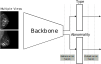
\includegraphics[width=.9\linewidth]{./images/model.png}
\caption{\label{fig:model}Our model takes as input a set of images that show several views of the same breast. We investigate on several fusion strategies (dashed columns): (1) Fuse features at bottleneck, and (2) fuse prediction outputs. We also set an auxiliary multi-label classification objective on abnormalities (bottom branch).}
\end{figure}

\subsection{Preprocessing, Training, and Validation}
\label{sec:org027e209}

We convert the original images given as DICOM series into 8-bit images,
and rescale these from \(1914 \times 2294\) to \(1024 \times 1024\) pixels. We found that this
is a good compromise as it conserves most fine-grained details while
reducing computational burden.

Next, we apply the triangle thresholding approach described in \autocite{walsh22}
to remove background noise.

Finally, we apply vertical mirroring to right breasts so as to align them with left breasts.

We feed our model with mini-batches that combine both views of a given breast, and
apply our fusion operators prior to computing the gradients.

Our classification tasks are optimized as follows:

\begin{enumerate}
\item \textbf{Type}: Classifies breasts as Malignant/Benign using a Binary Cross-Entropy.
\item \textbf{Abnormality}: Classifies breasts as Mass \textbf{and/or} calcification using a Binary Cross-Entropy
in a multi-label fashion, i.e. we apply the sigmoid operator to the outputs.
\end{enumerate}

We train both our backbone and classification heads in an end-to-end regime through
gradient descent using a cross-validation strategy.
We leverage the training/validation splits described in Sec. \ref{split}, and train for
of \(20\) epochs, where each epoch contains \(30\) randomly sampled mini-batches,
where each mini-batch contains \(16\) images, i.e. \(8\) breasts.

Our gradients are computed using the Adam optimizer with a learning rate of
\(5 \times 10^{-5}\).

When combining different objectives, we set weighing factors to
the losses to \(1\).

For comparison with the state-of-the-art \autocite{walsh22}, we select the model so
as to maximize the area under the curve (ROC).

\section{Results}
\label{sec:orgcf50070}


\printbibliography
\end{document}
